\fancyhead[RO]{\fontsize{8.5pt}{10pt}\selectfont\textsf{MỤC 1.1}\quad \textsf{Bốn cách biểu diễn một hàm số}\quad \textbf{\textsf{\thepage}}}

\noindent
\begin{minipage}[t]{0.265\textwidth}
    \fontsize{8pt}{10.2pt}\selectfont
    \begin{center}
        \textbf{\textsf{Bảng 2}}\quad \textsf{Dân số thế giới}\\[3pt]
        \renewcommand{\arraystretch}{1.08}
        \begin{tabular}{|c|c|}
            \hline
            \rowcolor{blue!10}
            \parbox[c]{1.6cm}{\centering $t$\\ \scriptsize (năm tính\\ \scriptsize từ 1900)} & 
            \parbox[c]{1.8cm}{\centering Dân số\\ \scriptsize (triệu người)} \\
            \hline
            0   & 1650 \\
            10  & 1750 \\
            20  & 1860 \\
            30  & 2070 \\
            40  & 2300 \\
            50  & 2560 \\
            60  & 3040 \\
            70  & 3710 \\
            80  & 4450 \\
            90  & 5280 \\
            100 & 6080 \\
            110 & 6870 \\
            \hline
        \end{tabular}
    \end{center}

    \vspace{8pt}
    \begin{center}
        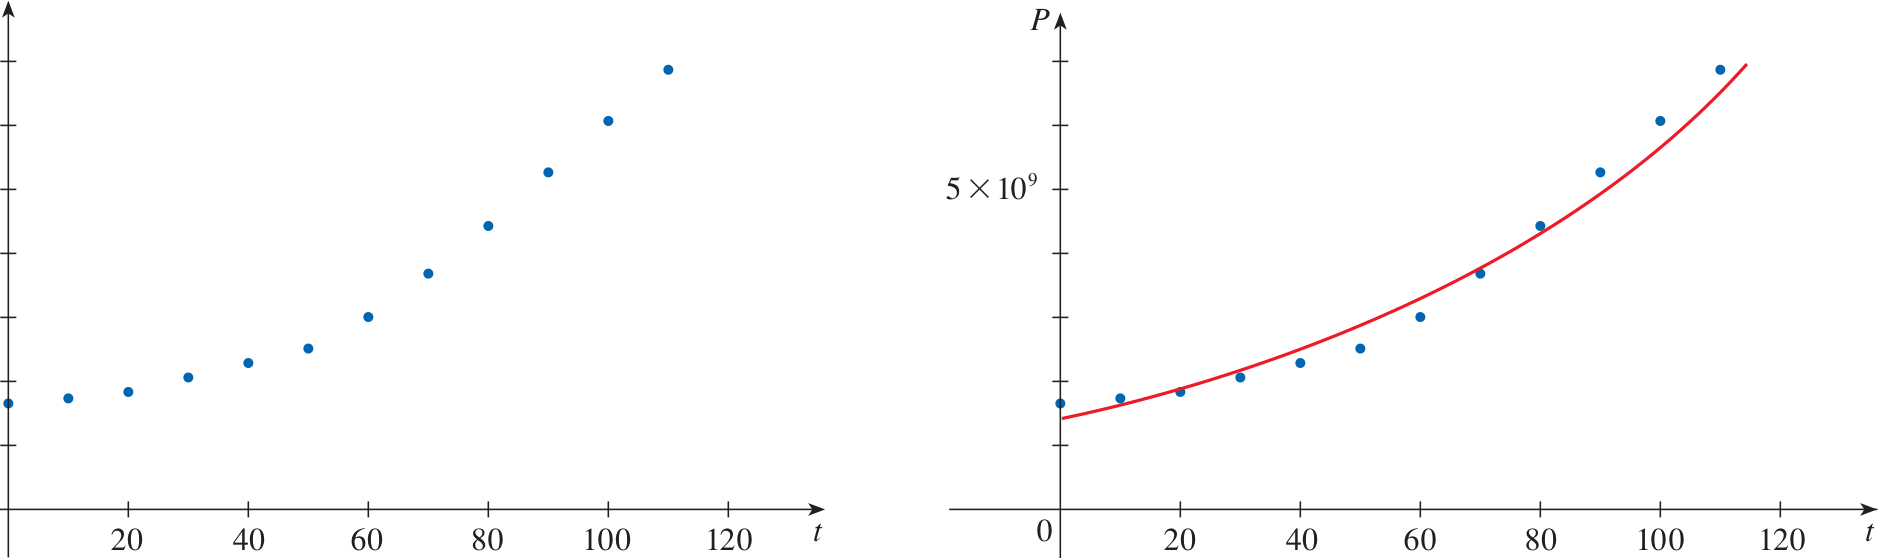
\includegraphics[width=0.92\linewidth]{images/p0046_fig9.png}\\[2pt]
        \textbf{\textsf{HÌNH 9}}
    \end{center}

    \vspace{6pt}
    \noindent
    Một hàm số được xác định bởi một bảng giá trị được gọi là một \emph{hàm dạng bảng} (tabular function).

    \vspace{8pt}
    \begin{center}
        \textbf{\textsf{Bảng 3}}\\[3pt]
        \renewcommand{\arraystretch}{1.1}
        \begin{tabular}{|c|c|}
            \hline
            \rowcolor{blue!10}
            $w$ (ounce) & $C(w)$ (đô la) \\
            \hline
            $0 < w \le 1$ & 1.00 \\
            $1 < w \le 2$ & 1.15 \\
            $2 < w \le 3$ & 1.30 \\
            $3 < w \le 4$ & 1.45 \\
            $4 < w \le 5$ & 1.60 \\
            $\cdot$       & $\cdot$ \\
            $\cdot$       & $\cdot$ \\
            \hline
        \end{tabular}
    \end{center}
\end{minipage}%
\hfill
\begin{minipage}[t]{0.708\textwidth}
    \fontsize{9.3pt}{13.2pt}\selectfont
    \noindent
    \textbf{A.} Biểu diễn hữu ích nhất của diện tích hình tròn theo bán kính có lẽ là công thức đại số $A = \pi r^2$ hoặc, dưới dạng ký hiệu hàm số, $A(r) = \pi r^2$. Ta cũng có thể lập một bảng giá trị hoặc phác họa đồ thị (một nửa parabol). Vì hình tròn phải có bán kính dương, nên tập xác định là $\{r \mid r > 0\} = (0, \infty)$ và tập giá trị cũng là $(0, \infty)$.

    \vspace{4pt}
    \noindent
    \textbf{B.} Ta được cho mô tả của hàm số bằng lời: $P(t)$ là dân số loài người trên thế giới tại thời điểm $t$. Hãy quy ước thời gian $t$ sao cho $t = 0$ tương ứng với năm 1900. Bảng 2 cung cấp một cách biểu diễn thuận tiện cho hàm số này. Nếu ta biểu diễn các cặp có thứ tự trong bảng lên hệ tọa độ, ta thu được đồ thị (gọi là \emph{biểu đồ phân tán} - scatter plot) ở Hình 9. Đây cũng là một cách biểu diễn hữu ích; đồ thị cho phép chúng ta nắm bắt toàn bộ dữ liệu chỉ trong một cái nhìn. Vậy còn một công thức thì sao? Dĩ nhiên, không thể thiết lập một công thức tường minh cho biết chính xác dân số loài người $P(t)$ tại bất kỳ thời điểm $t$ nào. Nhưng ta hoàn toàn có thể tìm được một biểu thức cho hàm số \emph{xấp xỉ} $P(t)$. Trên thực tế, bằng cách sử dụng các phương pháp được giải thích trong Mục 1.4, ta thu được một hàm xấp xỉ cho dân số $P$:
    \[
    P(t) \approx f(t) = (1{,}43653 \times 10^9) \cdot (1{,}01395)^t
    \]
    Hình 10 cho thấy rằng đây là một hàm “khớp” (fit) khá tốt. Hàm số $f$ được gọi là một \emph{mô hình toán học} (mathematical model) cho sự gia tăng dân số. Nói cách khác, đó là một hàm số có công thức tường minh mô phỏng hành vi của hàm số đã cho. Tuy nhiên, chúng ta sẽ thấy rằng các ý tưởng của giải tích có thể được áp dụng trực tiếp cho một bảng giá trị; một công thức tường minh không phải là điều bắt buộc.

    \begin{center}
        \begin{tikzpicture}[x=0.038\linewidth, y=0.48cm]
            \draw[->, >=stealth] (-6,0) -- (132,0) node[below left=2pt, font=\scriptsize] {$t$};
            \draw[->, >=stealth] (0,-0.3) -- (0,7.6) node[below left=2pt, font=\scriptsize] {$P$};
            
            \foreach \x in {20, 40, 60, 80, 100, 120} {
                \draw (\x, 0.12) -- (\x, -0.12) node[below, font=\scriptsize] {$\x$};
            }
            \node[below left=1pt, font=\scriptsize] at (0,0) {$0$};
            
            \foreach \y in {1, 2, 3, 4, 5, 6, 7} {
                \draw (1.5, \y) -- (-1.5, \y);
            }
            \node[left=2pt, font=\scriptsize] at (-1.5, 5) {$5 \times 10^9$};
            
            \node[below=13pt, font=\scriptsize] at (60,0) {Năm tính từ 1900};
            
            \foreach \px/\py in {0/1.65, 10/1.75, 20/1.86, 30/2.07, 40/2.30, 50/2.56, 60/3.04, 70/3.71, 80/4.45, 90/5.28, 100/6.08, 110/6.87} {
                \fill[blue!75!cyan] (\px, \py) circle (1.3pt);
            }
            
            \draw[thick, red, domain=0:115, samples=80, smooth] 
                plot (\x, {1.43653 * exp(\x * 0.0138538)});
        \end{tikzpicture}\\[2pt]
        \textbf{\textsf{HÌNH 10}}
    \end{center}

    \vspace{2pt}
    \noindent
    Hàm số $P$ là ví dụ điển hình cho các hàm số xuất hiện bất cứ khi nào chúng ta cố gắng áp dụng giải tích vào thế giới thực. Chúng ta bắt đầu bằng một mô tả bằng lời về một hàm số. Sau đó, ta có thể xây dựng một bảng giá trị của hàm số, có thể từ các số đọc trên thiết bị đo trong một thí nghiệm khoa học. Dù không có hiểu biết đầy đủ về mọi giá trị của hàm số, chúng ta sẽ thấy xuyên suốt cuốn sách này rằng ta vẫn có thể thực hiện các phép toán giải tích trên một hàm số như vậy.

    \vspace{4pt}
    \noindent
    \textbf{C.} Một lần nữa, hàm số lại được mô tả bằng lời: Gọi $C(w)$ là chi phí gửi một phong bì lớn có khối lượng $w$. Quy định mà Bưu chính Hoa Kỳ (US Postal Service) áp dụng từ năm 2019 như sau: Chi phí là 1 đô la cho tối đa 1 oz, cộng thêm 15 cent cho mỗi ounce (hoặc phần lẻ của ounce) tiếp theo cho đến 13 oz. Một bảng giá trị là cách biểu diễn thuận tiện nhất cho hàm số này (xem Bảng 3), mặc dù ta cũng có thể phác họa đồ thị của nó (xem Ví dụ 10).

    \vspace{4pt}
    \noindent
    \textbf{D.} Đồ thị trong Hình 1 là cách biểu diễn tự nhiên nhất cho hàm gia tốc thẳng đứng $a(t)$. Đúng là ta có thể lập một bảng giá trị, và thậm chí có thể thiết lập một công thức xấp xỉ. Nhưng tất cả những gì một nhà địa chất cần...
\end{minipage}